\chapter{Materials and Methods} \label{chap:Materials_and_Methods}

\textbf{WARUM NOCHMAL GENAU COSINUS?}

The tools used in this project were installed with the Conda package distribution system version 2-2.4.0 \autocite{anaconda_software_distribution_anaconda_2020}. With Conda, Python packages containing e.~g.~ full software tools can be managed by local environments for simple access without the necessity of a complex system-wide installation \autocite{anaconda_software_distribution_anaconda_2020}. Creation of an environment similar to the one used in this project, is possible with the conda environment creation from YAML file function, the results can be easily recreated on any modern UNIX-like operating system that has Conda installed. 

\begin{lstlisting}[language=sh]
git clone https://github.com/ahenoch/Masterthesis.git
cd Masterthesis
conda env create -f Environment.yml
\end{lstlisting}  

The YAML file containing the informations for installation like e.~g.~ the used tools versions is present in the \href{https://github.com/ahenoch/Masterthesis.git}{Projects GitHub Repository} an can be made available by e.~g.~ cloning the repository (the important packages and their related versions are also listed in \autoref{tab:Package_Version}).

\begin{table}[!hbt]
    \centering
    \caption[Package Version]{\textbf{Package Version.} The packages that need to be installed by Conda in a specific version for the pipeline to work as expected are listed in this table. Other related packages necessary for execution of the listed ones are meanwhile installed automatically by Conda.}
    \label{tab:Package_Version}
    \pgfplotstabletypeset[
        every head row/.style={
            before row={
                \toprule
            },
            after row={
                \midrule
            },
        },
        every last row/.style={
            after row={
                \bottomrule
            },
        },
        begin table=\begin{tabular*}{.5\textwidth},
        end table=\end{tabular*},
        columns={0,1,2},
        columns/0/.style={string type, multicolumn names=l,column name=\textbf{Name}, column type=@{\extracolsep{\fill}\hspace{6pt}}l},
        columns/1/.style={string type, multicolumn names=l,column name=\textbf{Version}, column type=l},
        columns/2/.style={string type, multicolumn names=l,column name=\textbf{Channel}, column type=l}
    ]
    {Graphics/Packages.csv}
\end{table}

Since its file size exceeds the limits of GitHub, the FASTA file containing all the known high quality sequences of the \gls{IAV}, that is used in this project must be manually retrieved in the latest version \footnote{GenBank Genome Sequence/Annotation Update >= 05/2021} from the \href{https://www.fludb.org/brc/home.spg?decorator=influenza}{\gls{IRD}}.

\begin{table}[!hbt]
    \centering
    \caption[Search Parameter for FASTA file]{\textbf{Search Parameter for FASTA file.} The parameters to use on the nucleotide sequence search interface of the \href{https://www.fludb.org/brc/home.spg?decorator=influenza}{Influenza Research Database}. All paremeters have to be precisely as listed for a exact replication of the FASTA file used in this project.}
    \label{tab:Search}
    \pgfplotstabletypeset[
        every head row/.style={
            before row={
                \toprule
            },
            after row={
                \midrule
            },
        },
        every last row/.style={
            after row={
                %... & ... & ... & ... & ... & ... & ... & ...\\
                \bottomrule
            },
        },
        begin table=\begin{tabular*}{.5\textwidth},
        end table=\end{tabular*},
        columns={0,1},
        columns/0/.style={string type, multicolumn names=l,column name=\textbf{Field}, column type=@{\extracolsep{\fill}\hspace{6pt}}l},
        columns/1/.style={string type, multicolumn names=l,column name=\textbf{Parameter}, column type=l},
    ]
    {Graphics/search.csv}
\end{table}

The FASTA file can be retrieved by navigating from \textit{SEARCH DATA} to \textit{Search Sequences} and then to \textit{Nucleotide Sequences}. On the following page the parameters given in \autoref{tab:Search} have to be used to request the correct file. Following the search request \textit{Select all X segments} have to be checked and after \textit{Download}, \textit{Segment FASTA} has to be checked in \textit{Specify Download Type} setting and \textit{Custom format - select fields from list} in \textit{Format for FASTA file definition line}. Accession Number, Strain Name, Segment, Protein Symbol, Type, SubType, Date, Host Species, Curation Flag have then to be added in the following order. After downloading the FASTA file it has to be placed as \textit{A.fasta} in the local root of the \href{https://github.com/ahenoch/Masterthesis.git}{Projects GitHub Repository}. The version used for the proposed results was acquired at 08/11/2020 \footnote{GenBank Genome Sequence/Annotation Update <= 11/2020 }. Newer versions might change the results slightly.

% \begin{enumerate}[noitemsep]
%     \item \textit{SEARCH DATA}
%     \item \textit{Search Sequences}
%     \item \textit{Nucleotide Sequences}
%     \item \textit{Data Type:} Genome Segments, \textit{Virus Type:} A, \textit{Complete Genome:} Complete Genome Only, \textit{Select Segments:} All, \textit{Complete:} All
%     \item \textit{Search}
%     \item \textit{Select all X segments}
%     \item \textit{Download}
%     \item \textit{Specify Download Type:} Segment FASTA
%     \item \textit{Format for FASTA file definition line:}  Custom format - select fields from list
%     \item \textbf{add in the following order:} Accession Number, Strain Name, Segment, Protein Symbol, Type, SubType, Date, Host Species, Curation Flag
%     \item save as A.fasta in the cloned Masterthesis folder
% \end{enumerate}
%or from the \href{https://github.com/ahenoch/Masterthesis.git}{Projects GitHub Repository}. Using the manually retrieved updated version of the FASTA file might change the recreated results slightly.

\begin{table}[!hbt]
    \centering
    \caption[Used Methods in a Nutshell]{\textbf{Used Methods in a nutshell.} For easier separation the different settings were listed. Method \acrshort{PCA}/\acrshort{DBCV} and \acrshort{PCA}/Knee use \autoref{fig:Vectorization_Pipeline} pathway \textsf{\textbf{1}} followed by \autoref{fig:Clustering_Pipeline} pathway \textsf{\textbf{3}} for method \acrshort{PCA}/\acrshort{DBCV} and \textsf{\textbf{4}} for \acrshort{PCA}/Knee. Method \acrshort{UMAP}/\acrshort{DBCV} and \acrshort{UMAP}/Knee differ only by the first part using \autoref{fig:Vectorization_Pipeline} pathway \textsf{\textbf{2}} instead of \textsf{\textbf{1}}.}
    \label{tab:methods}
    \pgfplotstabletypeset[
        every head row/.style={
            before row={
                \toprule
            },
            after row={
                \midrule
            },
        },
        every last row/.style={
            after row={
                \bottomrule
            },
        },
        begin table=\begin{tabular*}{\textwidth},
        end table=\end{tabular*},
        columns={0,1,2,3},
        columns/0/.style={string type,multicolumn names=l,column name=\textbf{Method}, column type=@{\extracolsep{\fill}\hspace{6pt}}l},
        columns/1/.style={string type,multicolumn names=l,column name=\textbf{100 Components}, column type=l},
        columns/2/.style={string type,multicolumn names=l,column name=\textbf{30 Components}, column type=l},
        columns/3/.style={string type,multicolumn names=l,column name=\textbf{Exploration}, column type=l}
    ]
    {Graphics/methods.csv}
\end{table}

In this project four different ways to cluster the segments of \gls{IAV} are described and discussed in the following (\autoref{tab:methods}). For the methods involving \gls{UMAP}, as well as the methods without \gls{UMAP}, one Jupyter Notebook with the settings and results for each is available in the \href{https://github.com/ahenoch/Masterthesis.git}{Projects GitHub Repository}. To access the Jupyter Notebooks holding the cluster and analysis pipeline, as well as recreate the results, the IPYNB Files in the \href{https://github.com/ahenoch/Masterthesis.git}{Projects GitHub Repository} have to be opened and started in a Jupyter Lab server \autocite{kluyver_jupyter_2016}. All discussed results in this project are related to the two Jupyter Notebooks and the settings and tools used in it.

\begin{lstlisting}[language=sh]
conda activate Masterthesis
jupyter lab
\end{lstlisting}  

A raw clustering tool for \gls{IAV} genomes that saves the results as CSV files and colored \gls{HDBSCAN} clustertrees using ETE3 version 3.1.2 is also available in the \href{https://github.com/ahenoch/Masterthesis.git}{Projects GitHub Repository} and is intended to be used in the future, with the best settings elaborated in this project \autocite{huerta-cepas_ete_2016}. It is designed to function as a clustering tool, without the need of a running Jupyter Lab server and with easier modification and faster execution in mind (\autoref{fig:Vectorization_Pipeline} and \autoref{fig:Clustering_Pipeline}). Many settings to be used to cluster \gls{IAV} are already included and other functions can be added with ease.

\begin{lstlisting}[language=sh]
conda activate Masterthesis
python3 Clustering.py -i A.fasta -o PCA_raw -p 50
\end{lstlisting}  

All settings available to the present day are listed on the next page.

\begin{leftbar}
    \textbf{Clustering.py}
    \begin{nstabbing}
        \qquad\=\qquad\qquad\qquad\qquad\quad\=\kill
    
        -i \> -{}-{}infile \> [path to input file (e.~g.~ A.fasta)]\\
        
        -o \> -{}-{}outfolder \> [path to input file (default: Results)]\\
        
        -s \> -{}-{}segments \> [segments to run the pipeline on (default: 1 2 3 4 5 6 7 8)]\\
        
        -c \> -{}-{}custom\_header \> [if using FASTA with a custom header, every part of it has\\
        
        \> \> to be declared (default: accession strain segment protein\\
        
        \> \> genus subtype date host curation genome)]\\
        
        -m \> -{}-{}metric \> [metric to use in the pipeline (default: cosine)]\\
        
        -mc \> -{}-{}min\_clust \> [min\_cluster\_size parameter for HDBSCAN (default: 2)]\\
        
        -ms \> -{}-{}min\_sample \> [min\_samples parameter for HDBSCAN (default: 1)]\\
        
        -n \> -{}-{}neigbors \> [n\_neighbors parameter for UMAP (default: 100)]\\
        
        -u \> -{}-{}umap \> [n\_components parameter for UMAP (optional)]\\
        
        -p \> -{}-{}pca \> [n\_components parameter for PCA (optional)]\\
        
        -k \> -{}-{}max\_kneedle \> [ (default: 500)]\\
        
        -r \> -{}-{}render \> [ (default: 'svg')]\\
        
        -e \> -{}-{}epsilon \> [ (default: 'kneedle')]
    \end{nstabbing}
\end{leftbar}

\begin{figure}[!hbt]
    \centering
    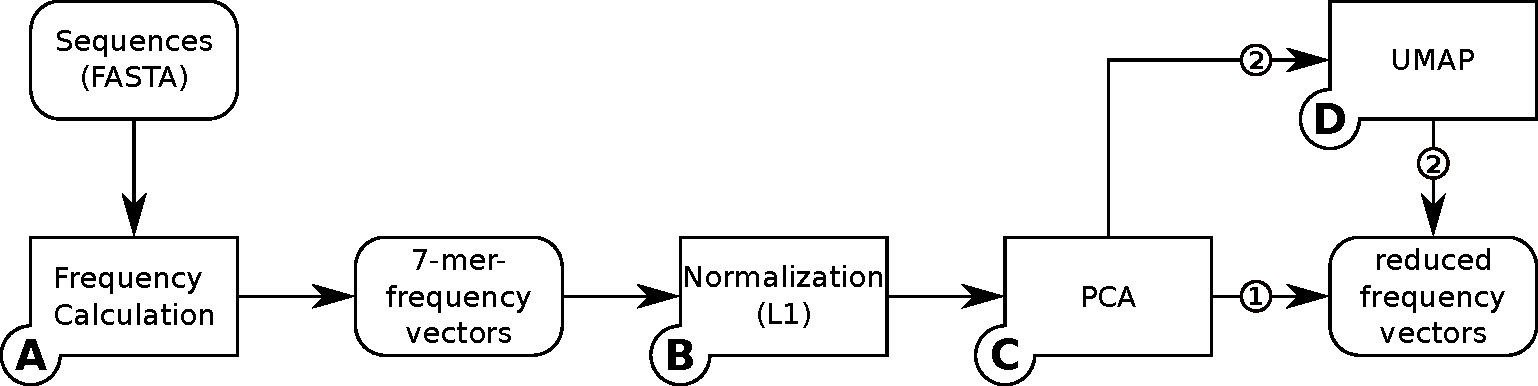
\includegraphics[width=\textwidth]{Graphics/Vectorization.pdf}
    \caption[Clustering Pipeline]{\textbf{Vectorization Pipeline.} The vectorization pipeline of the proposed clustering tool. The FASTA file is translated to vectors containing the k-mer frequencies of the specific sequence (\autoref{sec:Frequency}). As shown in pathway \textsf{\textbf{1}}, by normalization with L1-norm and \gls{PCA} a low complexity representation of the vectors is obtained for clustering (\autoref{sec:Normalization} and \autoref{sec:PCA}). Pathway \textsf{\textbf{2}} describes additional execution of \gls{UMAP} that can be used after \gls{PCA} as intermediate instead of final step (\autoref{sec:UMAP}).}
    \label{fig:Vectorization_Pipeline}
\end{figure}

\begin{figure}[!hbt]
    \centering
    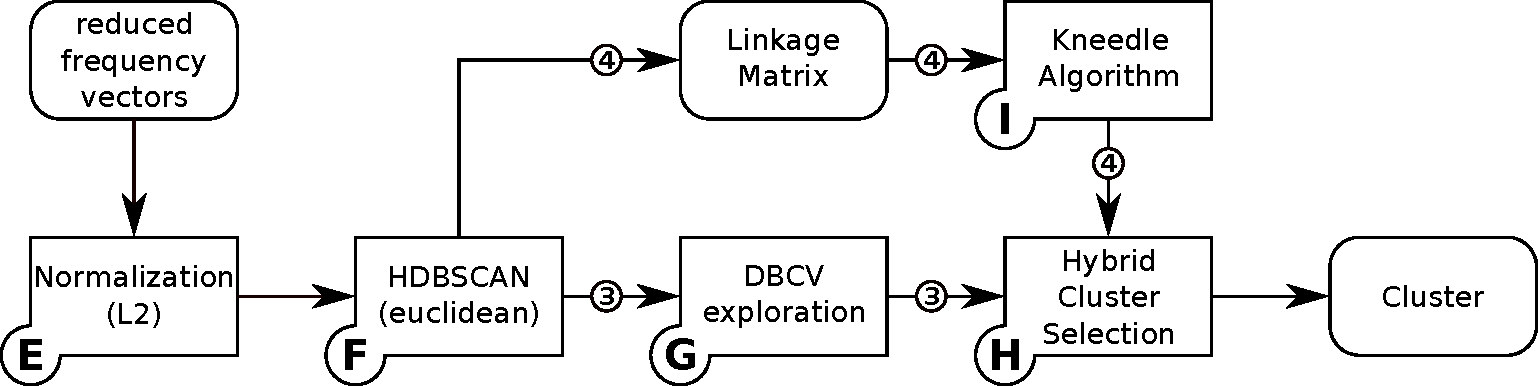
\includegraphics[width=\textwidth]{Graphics/Clustering.pdf}
    \caption[Clustering Pipeline]{\textbf{Clustering Pipeline.} Following the vectorization pipeline (\autoref{fig:Vectorization_Pipeline}) normalization is used again with L2-norm as preparation for \gls{HDBSCAN} (\autoref{sec:Normalization} and \autoref{sec:HDBSCAN}) Final hybrid clustering (\autoref{sec:HDBSCAN}) is prepared either with the Kneedle Algorithm (pathway \textsf{\textbf{4}} and \autoref{sec:Kneedle}) or DBCV exploration (pathway \textsf{\textbf{3}} and \autoref{sec:HDBSCAN}).}
    \label{fig:Clustering_Pipeline}
\end{figure}

\begin{figure}[!hbt]
    \centering
    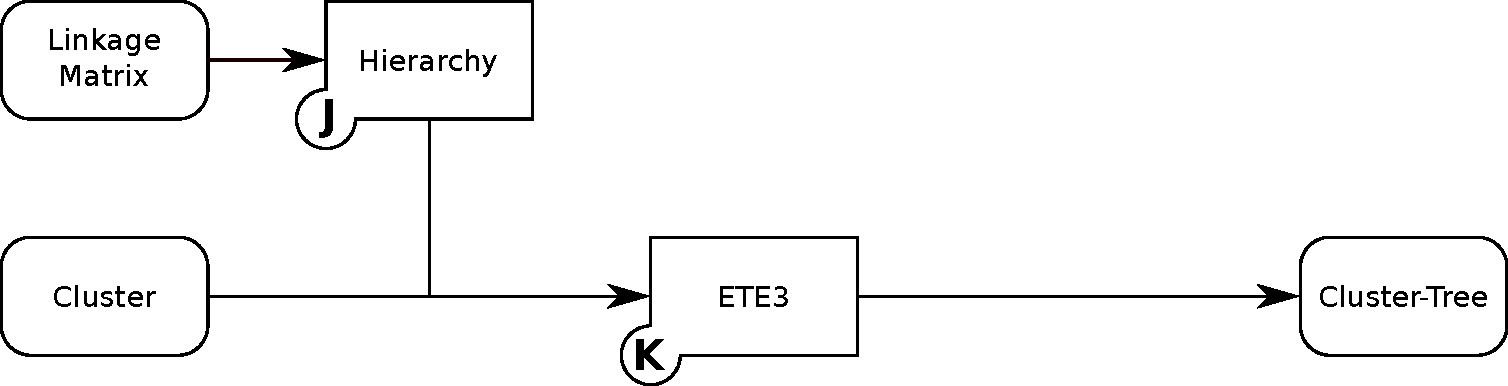
\includegraphics[width=\textwidth]{Graphics/Tree.pdf}
    \caption[Tree Building Pipeline]{\textbf{Tree Building Pipeline.} Following the clustering pipeline (\autoref{fig:Clustering_Pipeline}) the cluster-tree for visualization is build by ETE3 with the help of \textbf{hierarchy} function from the \textbf{scipy} package \autocite{huerta-cepas_ete_2016, scipy_10_contributors_scipy_2020}. To determine the centroids, for every cluster the normalized frequency vector (\autoref{fig:Clustering_Pipeline}) with the smallest distance to the other cluster members is calculated with the \textbf{spatial.distance.cdist} function also from the \textbf{scipy} package \autocite{scipy_10_contributors_scipy_2020}.}
    \label{fig:Tree_Pipeline}
\end{figure}

The tool takes around one hour to cluster all eight segments of \gls{IAV} and create the output in form of tables and clustertree graphics with the suggested settings. 

\nopagebreak[1]

\section{K-Mer Frequency} \label{sec:Frequency}

The FASTA file containing the to be clustered genomes of \gls{IAV} were translated to vectors for clustering in high dimension by counting their 7-mer frequency (\autoref{fig:Vectorization_Pipeline} \textsf{\textbf{A}}). Let $A$ be a mathematical sequence of all permutations with repetition of the set $\{A,C,G,T\}$ to the magnitude of seven, thus $m = 4^7$ elements (\autoref{eq:alphabet}) and $S$ a mathematical sequence of all $n$ genome sequences of one segment of \gls{IAV} in the FASTA file (\autoref{eq:alphabet}).

\begin{empheq}{alignat = -1}
    &A &&= ( \text{AAAAAAA} , \text{AAAAAAC} , \text{AAAAAAG} , \ldots , \text{TTTTTTT} &&)\label{eq:alphabet}\\
    &S &&= ( \text{GCAAAA...} , \text{GCAAAA...} , \text{AGCAAA...} , \ldots , \text{ATGGC...} &&)\label{eq:sequences}
\end{empheq}

The elements of $A$ represent all possible constellations of 7-mers. For the sequence $S_i$ let $s$ be the k-mer representation of that sequence with $l$ components. The vector component $x_{i,j}$ of a genome sequence $S_i$ was calculated by summing up the number of occurrences of element $A_j$ in all the 7-mers of genome sequence $S_i$ (\autoref{eq:frequency}). 

\begin{empheq}{alignat = -1}
    &x_{i,j} = \sum^l_{k=1} \delta(s_k, A_j), \quad i = 1, \ldots, n, \ j = 1, \ldots, m, \ \delta(s_k,A_j)=\left\{ \begin{array}{c}1\text{ if \ensuremath{s_k=A_j}}\\0\text{ if \ensuremath{s_k\neq A_j}}\end{array}\right.\label{eq:frequency}
\end{empheq}

This calculation was repeated for all of the $4^7$ elements of $A$, as well as for all sequences of $S$, building the matrix $\mathbf{X} = [ x_{i,j} ]$, holding the k-mer frequency vectors of the genome sequences of $S$ (\autoref{eq:full_matrix}).

\begin{empheq}{alignat = -1}
    &\mathbf{X} = \begin{bmatrix}x_{1,1} & x_{1,2} & x_{1,3} & \dots & x_{1,4^7}\\
    x_{2,1} & x_{2,2} & x_{2,3} & \dots & x_{2,4^7}\\
    x_{3,1} & x_{3,2} & x_{3,3} & \dots & x_{3,4^7}\\
    \vdots & \vdots & \vdots & \ddots & \vdots\\
    x_{i,1} & x_{i,2} & x_{i,3} & \dots & x_{i,4^7}
    \end{bmatrix}\label{eq:full_matrix}
\end{empheq}

The entries in the $j$ columns represent the number of occurencences of 7-mer $A_j$ in a genome sequence $S_i$. The rows represent the $i$ genome sequences from $S$ with it's frequency numbers. In summary e.~g.~ $x_{1,1}$ represents the number of occurences of the first 7-mer $A_1$ in the first genome sequence $S_1$.

A k-mer length of seven was used to make the method usable on machines with at least 32Gb of RAM while still being as accurate as possible. With 7-mers, $4^7$ possible combinations can occure, which has a lower chance of accidental matching combinations by e.~g.~ \glspl{SNP} then using 6-mers with only $4^6$ different possible constellations. Using 8-mers on the other hand increases the necessary RAM drastically, by building a matrix e.~g.~ for segment 4, $\mathbf{X}$ of size $56617 \times 4^8$ of 64 bit float numbers making $\approx$ 29.684Gb. Adding the necessary space for dimension reduction methods and other calculations 32Gb would be exceeded by far. 

\section{Normalization} \label{sec:Normalization}

The matrix $\mathbf{X}$ was normalized row-wise with the L1-norm to align the k-mer frequency vectors located in the rows to an equal length of one (\autoref{fig:Vectorization_Pipeline} \textsf{\textbf{B}}) (\autoref{eq:l1_norm} to \autoref{eq:l1_result}). The \textbf{preprocessing.normalize} function from the \textbf{scikit-learn (sklearn)} package, with \colorbox{backcolour}{norm='l1'} setting was used for the normalization \autocite{pedregosa_scikit-learn_2011}.

%\begin{lstlisting}[language=python]
%sklearn.preprocessing.normalize(M, norm='l1')
%\end{lstlisting}  

\begin{empheq}{alignat = -1}
    \mathbf{\hat{X}}_i &= \frac{\mathbf{X}_i}{\Vert\mathbf{X}_i\Vert_1} \label{eq:l1_norm}
\end{empheq}

\begin{empheq}{alignat = -1}
    \Vert\mathbf{\hat{X}}_i\Vert_1 &= 1\label{eq:l1_result}
\end{empheq}

The parameters used in this project with settings varying from the default are listed below. All available settings can be fount in the \href{https://scikit-learn.org/stable/modules/generated/sklearn.preprocessing.normalize.html}{API}

\begin{leftbar}
    \textbf{sklearn.preprocessing.normalize}
    \begin{nstabbing}
        \qquad\qquad\qquad\qquad\qquad\quad\=\kill
        
        X \> [Input matrix to be normalized]\\
        
        norm \> [Norm used for normalization (default: ’l2’)]
        
    \end{nstabbing}
\end{leftbar}

Due to an open\footnote{last accessed 02/06/21} \href{https://github.com/scikit-learn-contrib/hdbscan/issues/69}{issue} in the GitHub Repository of \gls{HDBSCAN} normalization with \textbf{preprocessing.normalize} was again used with the \colorbox{backcolour}{norm='l2'} setting, right before clustering. (\autoref{fig:Clustering_Pipeline} \textsf{\textbf{D}}). It was stated, normalization with L2-norm prior to clustering with euclidean metric setting, chord distance, which is also not directly available, can be used to approximate cosine distance.

\begin{figure}[!hbt]
    \centering
    %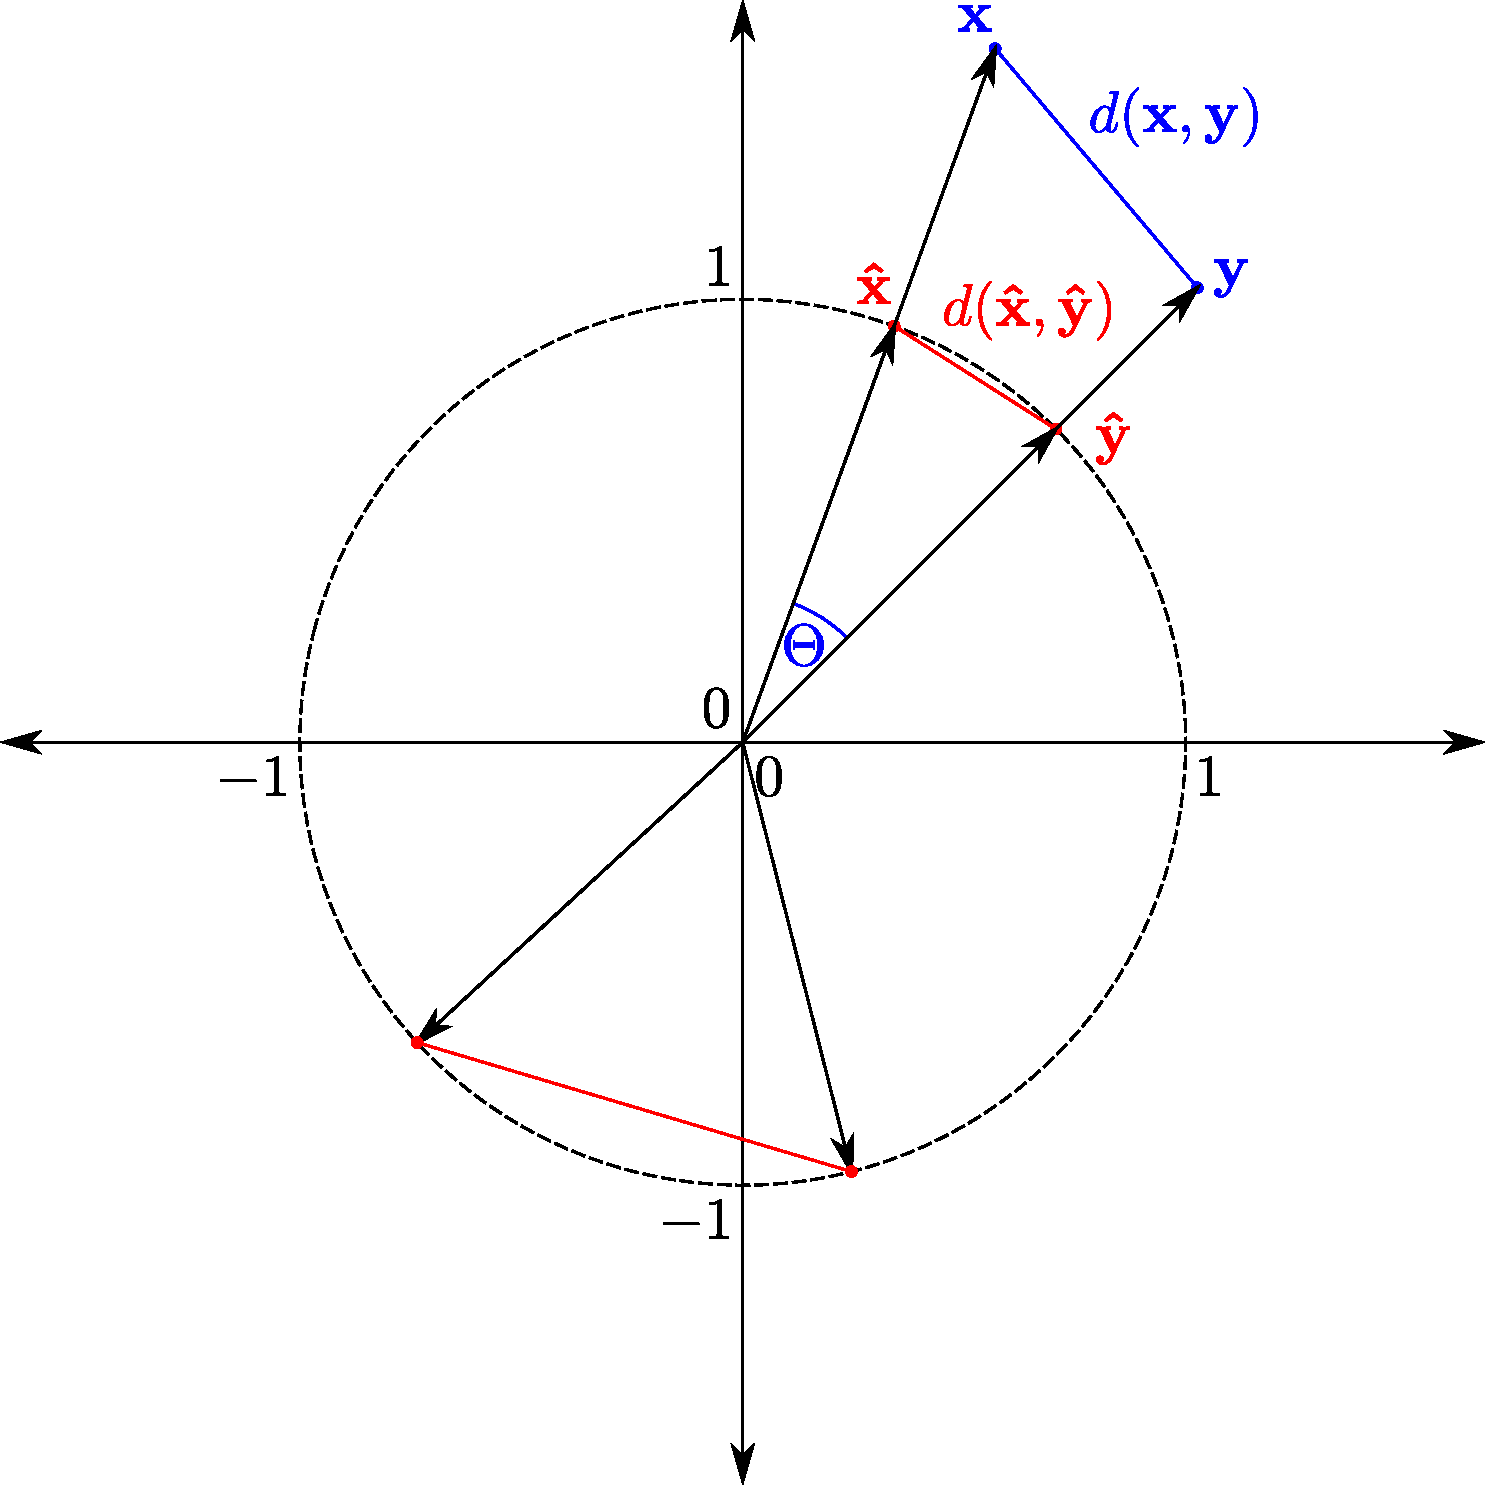
\includegraphics[width=\dimexpr\textwidth-2\fboxsep-2\fboxrule,fbox]{Graphics/L2_Euclidean.pdf}
    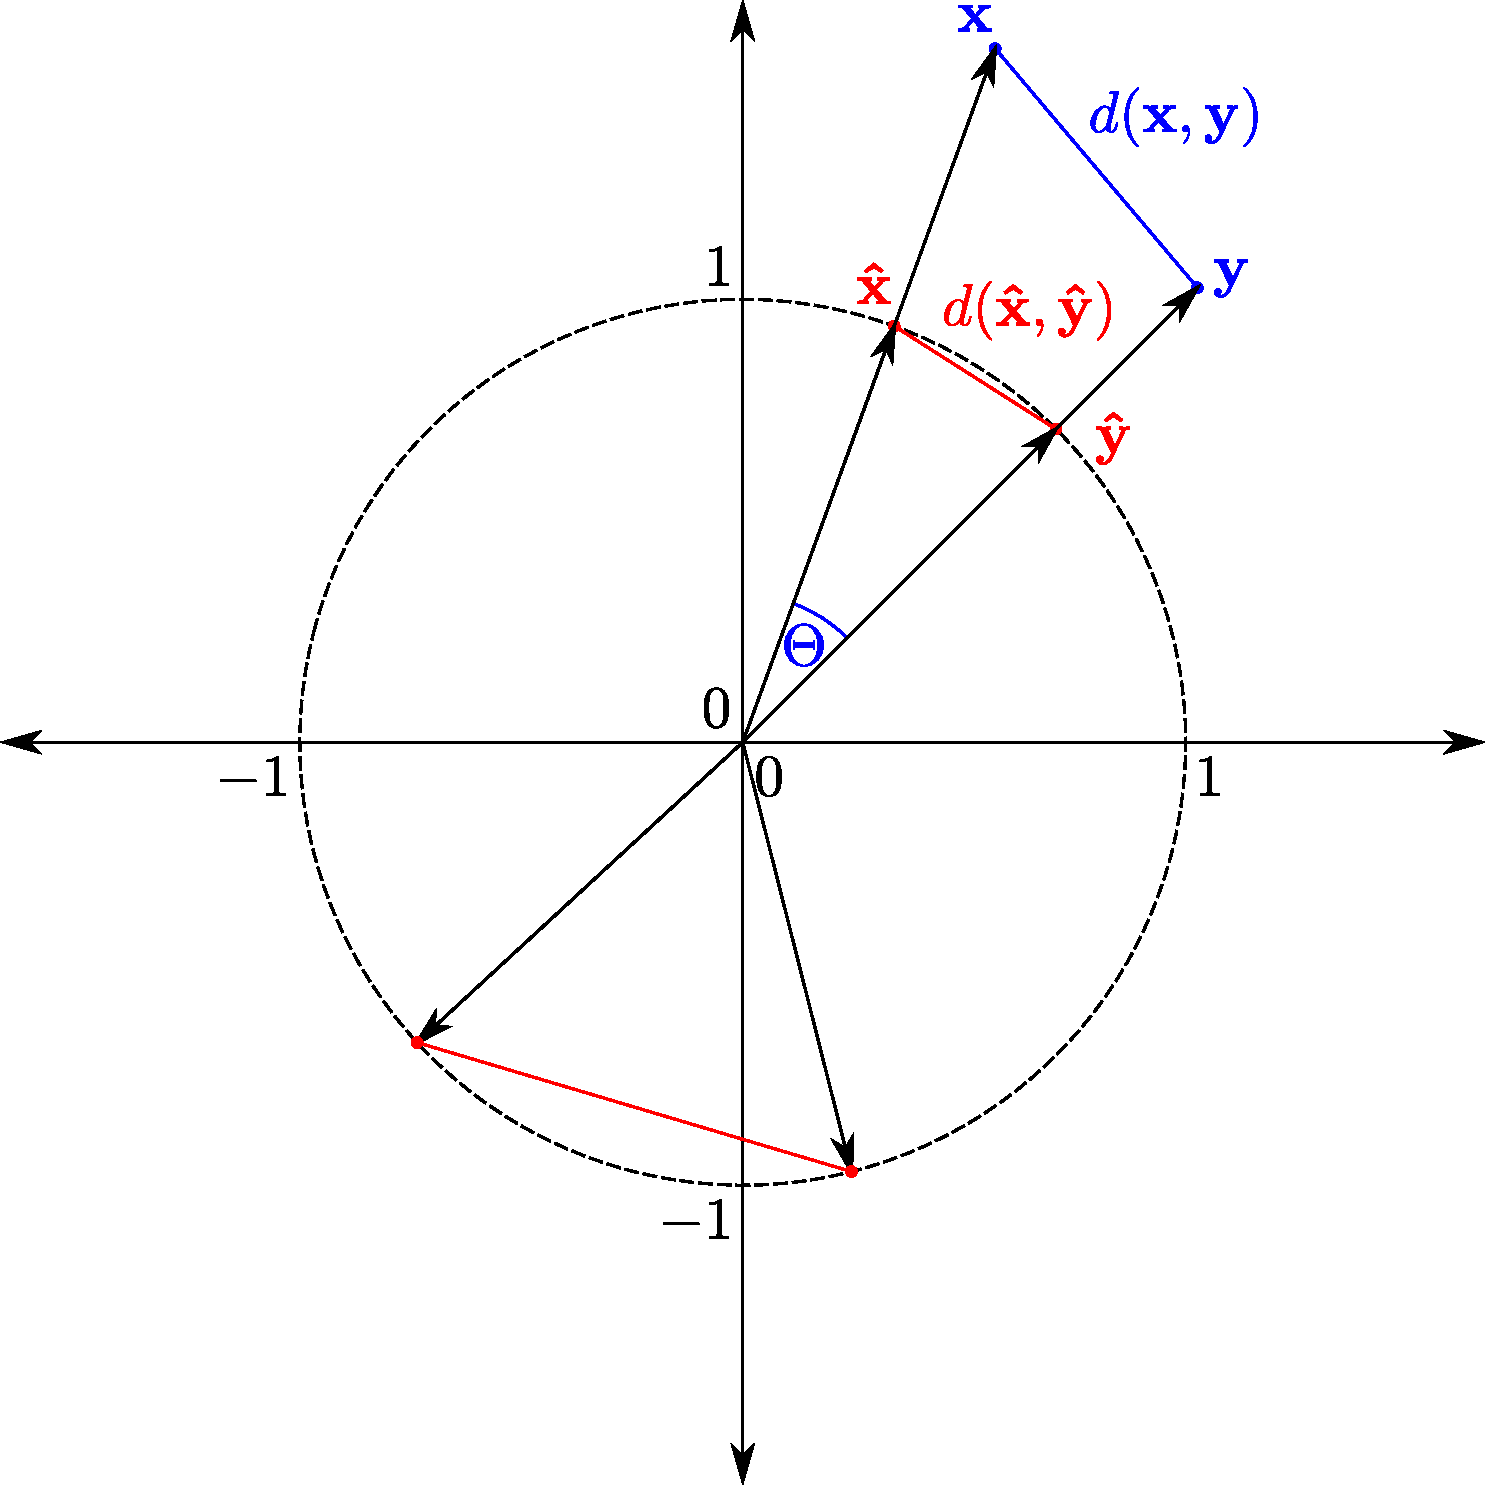
\includegraphics[width=\textwidth]{Graphics/L2_Euclidean.pdf}
    \caption[Graphical Background of L2 Normalisation]{\textbf{Graphical Background of L2 Normalisation.} .}
    \label{fig:L2_Normalisation_Background}
\end{figure}

Chord distance $d_{\text{chord}}$ can be calculated when having two vectors, here as an exmaple named as $\mathbf{x}'$ and $\mathbf{y}'$ with the same L2-norm equal to a radius $r$ of a sphere  centered to the origin of the coordinate system and an angle of $\Theta'$ (\autoref{eq:chord} and \autoref{fig:L2_Normalisation_Background}). The euclidean distance $d_{\text{eucl}}$ is equal to the chord distance for the same vectors $\mathbf{x}'$ and $\mathbf{y}'$ L2-norm $r$.

\begin{empheq}{alignat = -1}
    &\Vert\mathbf{x}'\Vert_2 = \Vert\mathbf{y}'\Vert_2 = r &&\to d_{\text{chord}}(\mathbf{x}',\mathbf{y}') &&= 2 \cdot r \sin \left(\frac{\Theta'}{2}\right) \vee\label{eq:chord}\\
    &\Vert\mathbf{x}'\Vert_2 = \Vert\mathbf{y}'\Vert_2 = r &&\to d_{\text{chord}}(\mathbf{x}',\mathbf{y}') &&= d_{\text{eucl}}(\mathbf{x}',\mathbf{y}')\\
    &&&&&= \Vert\mathbf{x}' - \mathbf{y}'\Vert_2
\end{empheq}

Thus in this project chord distance can be calculated with the euclidean distance metric, posterior to the normalization with the L2-norm, which scales the vectors to the unit sphere (\autoref{eq:chord_eucl_1} to \autoref{eq:chord_eucl_2} and \autoref{fig:L2_Normalisation_Background}).

\begin{empheq}{alignat = -1}
    &\Vert\mathbf{\hat{x}}\Vert_2 = \Vert\mathbf{\hat{y}}\Vert_2 = 1 &&\to d_{\text{chord}}(\mathbf{\hat{x}},\mathbf{\hat{y}}) &&= d_{\text{eucl}}(\mathbf{\hat{x}},\mathbf{\hat{y}})\label{eq:chord_eucl_1}\\
    &&&&&= \Vert\mathbf{\hat{x}} - \mathbf{\hat{y}}\Vert_2 \label{eq:chord_eucl_2}
\end{empheq}

The used chord distance is proportional with the initially intended to use cosine distance as shown in \autoref{eq:chord_cos_1} to \autoref{eq:chord_cos_7}. Dividing the squared chord distance by 2 results in the cosinus distance of the vectors.

\begin{empheq}{alignat = -1}    
    &\Vert\mathbf{\hat{x}}\Vert_2 = \Vert\mathbf{\hat{y}}\Vert_2 = 1 &&\to d_{\text{chord}}(\mathbf{\hat{x}},\mathbf{\hat{y}})^2 &&= \Vert\mathbf{\hat{x}} - \mathbf{\hat{y}}\Vert_2^2\label{eq:chord_cos_1}\\
    &&&&&= (\mathbf{\hat{x}} - \mathbf{\hat{y}})^\top (\mathbf{\hat{x}} - \mathbf{\hat{y}})\label{eq:chord_cos_2}\\
    &&&&&= \mathbf{\hat{x}}^\top \mathbf{\hat{x}} - 2 \mathbf{\hat{x}}^\top \mathbf{\hat{y}} + \mathbf{\hat{y}}^\top \mathbf{\hat{y}}\label{eq:chord_cos_3}\\
    &&&&&= 2 - 2\mathbf{\hat{x}}^\top \mathbf{\hat{y}}\label{eq:chord_cos_4}\\
    &&&&&= 2 - 2 \cos(\Theta)\label{eq:chord_cos_5}\\
    &&&&&= 2 \cdot (1 - \cos(\Theta))\label{eq:chord_cos_6}\\
    &&&&&= 2 \cdot d_{\text{cos}}(\mathbf{x},\mathbf{y})\label{eq:chord_cos_7}
\end{empheq}

 Approximation of cosine distance by normalization with L2-norm followed by euclidean distance calculation is thus a possible and in this project used workaround to overcome the impossibility to use cosine distance.

\section{PCA} \label{sec:PCA}

To handle the complexity of the datasets generated in the project, as well as to simplify them with the least loss of information as possible \gls{PCA} was used (\autoref{fig:Clustering_Pipeline} \textsf{\textbf{C}}) \autocite{pearson_liii_1901}.\gls{PCA} is a statistical technique, used to find a new presentation of the dataset with a lower complexity by variance maximizing, uncorrelated variables, the \glspl{PC}, which are linear functions of the previous ones \autocite{jolliffe_principal_2016}. 

For the \gls{PCA} of matrix $\mathbf{X}$ the \textbf{decomposition.PCA} function from the \textbf{scikit-learn (sklearn)} package, with \colorbox{backcolour}{n\_components=30} setting was used \autocite{pedregosa_scikit-learn_2011}.

The matrix of $\mathbf{X}$ for e.g. segment 4 of \gls{IAV} is of size $56617 \times 4^7$ and the number of components to extract 30 of $4^7$ thereby $\approx 0.18\%$. The size limit of the \textbf{decomposition.PCA} function for calculation with default setting \colorbox{backcolour}{svd\_solver='auto'} is $500 \times 500$ and min. 80\% of the smallest dimension of components to extract. Thus \colorbox{backcolour}{svd\_solver='randomized'} setting of \textbf{decomposition.PCA} is used automatically \autocite{pedregosa_scikit-learn_2011}. Randomized truncated \gls{SVD} is calculated by \textbf{decomposition.PCA} as described in \textcite{halko_finding_2010}.

\autoref{eq:PCA_k} and \autoref{eq:PCA_30} denote the use of the \gls{PCA} by the method of \textcite{halko_finding_2010} to reduce the matrix $\mathbf{X}$ with $j=4^7$ dimensions to $k=30$ dimensions and the settings for the Jupyter results with the use of \gls{PCA} only \autocite{kluyver_jupyter_2016, jolliffe_principal_2016, pedregosa_scikit-learn_2011}.

\begin{empheq}{alignat = -1}
    &\mathbf{X}_{(k)} &&= \text{PCA}(\mathbf{X}, k)\label{eq:PCA_k}\\
    &\mathbf{X}_{(30)} &&= \text{PCA}(\mathbf{X}, 30)\label{eq:PCA_30}
\end{empheq}

The number of components to extract was selected by running \gls{PCA} with different settings for \colorbox{backcolour}{n\_components} with matrix $\mathbf{X}$ of segment 4 and comparing the sum of explained variance. Because of the high increase of explained variance from 10 to 20 and also from 20 to 30 components, a value of 30 was used as default in this project. A fairly small value was used, due to increasing computational effort of \gls{PCA} and also to preserve the usability of Spanning Tree calculation with \gls{HDBSCAN} (\autoref{tab:PCA_Dimension}).

\begin{table}[!hbt]
    \centering
    \caption[Explained Variance by different PCA settings]{\textbf{Explained Variance by different PCA settings.}.}
    \label{tab:PCA_Dimension}
    \pgfplotstabletypeset[
        every head row/.style={
            before row={
                \toprule
            },
            after row={
                \midrule
            },
        },
        every last row/.style={
            after row={
                \bottomrule
            },
        },
        begin table=\begin{tabular*}{.5\textwidth},
        end table=\end{tabular*},
        columns={0,1},
        columns/0/.style={int detect, multicolumn names=l,column name=\textbf{\#Components}, column type=@{\extracolsep{\fill}\hspace{6pt}}r},
        columns/1/.style={multicolumn names=l,column name=\textbf{Explained Variance}, column type=r}
    ]
    {Graphics/PCA.csv}
\end{table}

% Let $\mathbf{S}$ be a square covariance matrix of size $i \times i$, calculated on the dataset matrix $\mathbf{X}$ with $i$ $j$-dimensional vectors (size $i \times j)$. 

% \autocite{jolliffe_principal_2016}.

% \begin{empheq}{alignat = -1}
%     x^\ast_{i,j} = x_{i,j} - \bar{x}_j
% \end{empheq}

% \begin{empheq}{alignat = -1}
%     &\mathbf{X}^\ast &&= \mathbf{U} \mathbf{L} \mathbf{A}^\top\\
%     &&&= \mathbf{Y}
% \end{empheq}

% \begin{empheq}{alignat = -1}
%     &\mathbf{X}^{\ast^\top} \mathbf{X}^\ast &&= (\mathbf{U} \mathbf{L} \mathbf{A}^\top)^\top (\mathbf{U} \mathbf{L} \mathbf{A}^\top)\\
%     &&&= \mathbf{A}\mathbf{L}\mathbf{U}^\top\mathbf{U} \mathbf{L} \mathbf{A}^\top\\
%     &&&= \mathbf{A}\mathbf{L}^2\mathbf{A}^\top 
% \end{empheq}

% \begin{empheq}{alignat = -1}
%     \mathbf{Y}_{30} = \mathbf{U}_{30} \mathbf{L}_{30} \mathbf{A}_{30}^\top
% \end{empheq}

The parameters used in this project with settings varying from the default are listed below. All available settings can be fount in the
\href{https://scikit-learn.org/stable/modules/generated/sklearn.decomposition.PCA.html}{API} \autocite{pedregosa_scikit-learn_2011}.

% \begin{empheq}{alignat = -1}
%     &\mathbf{X} = \begin{bmatrix}x_{1,1} & x_{1,2} & x_{1,3} & \dots & x_{1,30}\\
%     x_{2,1} & x_{2,2} & x_{2,3} & \dots & x_{2,30}\\
%     x_{3,1} & x_{3,2} & x_{3,3} & \dots & x_{3,30}\\
%     \vdots & \vdots & \vdots & \ddots & \vdots\\
%     x_{i,1} & x_{i,2} & x_{i,3} & \dots & x_{i,30}
%     \end{bmatrix}\label{eq:full_matrix_2}
% \end{empheq}

\begin{leftbar}
    \textbf{sklearn.decomposition.PCA}
    \begin{nstabbing}
        \qquad\qquad\qquad\qquad\qquad\quad\=\kill

        svd\_solver \> [Strategy used to solve the \gls{SVD} (default: auto)]\\
        n\_components \> [Number of components to extract (default: None)]
    \end{nstabbing}
\end{leftbar}

\section{UMAP} \label{sec:UMAP}

\blindtext
\autocite{mcinnes_umap_2020}

The parameters used in this project with settings varying from the default are listed below. All available settings can be fount in the \href{https://umap-learn.readthedocs.io/en/latest/api.html}{API}.

\begin{leftbar}
    \textbf{umap.UMAP}
    \begin{nstabbing}
        \qquad\qquad\qquad\qquad\qquad\quad\=\kill

        n\_neighbors \> (default: 15)\\
        
        min\_dist \> (default: 0.1)\\
        
        n\_components \> (default: 2)\\
        
        metric \> (default: 'euclidean')
    \end{nstabbing}
\end{leftbar}



\section{Hierarchical Density-Based Spatial Clustering of Applications with Noise} \label{sec:HDBSCAN}

\gls{HDBSCAN} was used to cluster the reduced vectors \autoref{fig:Clustering_Pipeline} \textsf{\textbf{F}}). It is an clustering algorithm proposed by \textcite{campello_hierarchical_2015} as a novel version of the well-known \gls{DBSCAN} \autocite{hutchison_density-based_2013}. Execution of \gls{HDBSCAN} involves varying values of $\varepsilon$, thus, not one specific threshold is used to define the clusters, but instead clusters of varying densities are extracted based on their stability over epsilon \autocite{mcinnes_hdbscan_2017}. 

As proposed in \textcite{malzer_hybrid_2020}, by combining \gls{HDBSCAN} with \gls{DBSCAN}, some of the disadvantages of using either of these methods can be avoided \autocite{mcinnes_hdbscan_2017, moulavi_density-based_2014}. Since \gls{DBSCAN} is a hierarchical clustering tool, it is dependent on a strict threshold for clustering. Points not included in this threshold value are omitted and not clustered \autocite{ester_density-based_1996, schubert_dbscan_2017}. \gls{HDBSCAN}, on the other hand, tend to create unwanted micro-clusters in areas of high density \autocite{mcinnes_hdbscan_2017}. Using the hybrid approach proposed in \autocite{malzer_hybrid_2020}, a threshold value $\varepsilon$ can be used to extract these high density areas as single clusters with \gls{DBSCAN}, but still use the method of \gls{HDBSCAN} for the otherwise omitted points (\autoref{fig:Hybrid}). This method is useful when having a small cluster size value, while still aiming to cluster high-density areas together exactly suitable for the proposed clustering. Specific strains of \gls{IAV} are sequenced a lot more, thereby probably creating high-density areas that should be clustered together with \gls{DBSCAN}. The small cluster size is, thereby, used to find small clusters of rare sequenced variants by \gls{HDBSCAN}, with possibly important mutations in low-density areas \autocite{malzer_hybrid_2020}. As explained, the smallest minimum cluster size of 2 was used to capture, in the best case, even genomes with single \glspl{SNP} at rare appearing positions, in their own clusters. To declare as least points as possible as noise, the minimum samples value was also set to the minimum 1. 

Distance calculations by \gls{HDBSCAN} were performed with the euclidean distance setting due to an open issue in the GitHub Repository of \gls{HDBSCAN}\footnote{\url{https://github.com/scikit-learn-contrib/hdbscan/issues/69 (last accessed 06/02/21)}}. In the issue the inability to use cosine distance metric with \gls{HDBSCAN} and the approximation of it by chord distance metric, was described. Given that chord distance metric is also not available firsthand, it was also mentioned, that it can be used by normalization of the dataset with L2-norm, prior to clustering with euclidean metric setting \autoref{fig:Clustering_Pipeline} \textsf{\textbf{E}}). 

\begin{figure}[!hbt]
    \centering
    \begin{subfigure}[b]{0.475\textwidth}
        \caption[Chord]{\textbf{Chord}}
        \label{subfig:Chord}
        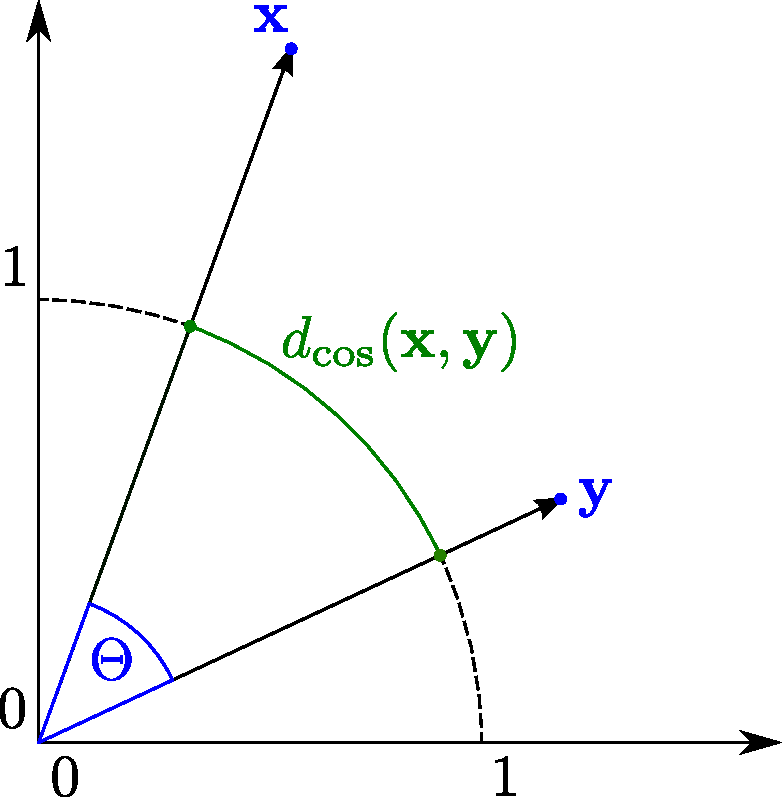
\includegraphics[width=\textwidth]{Graphics/Chord.pdf}
    \end{subfigure}
    \hfill
    \begin{subfigure}[b]{0.475\textwidth}
        \caption[L2]{\textbf{L2}}
        \label{subfig:L2}            
        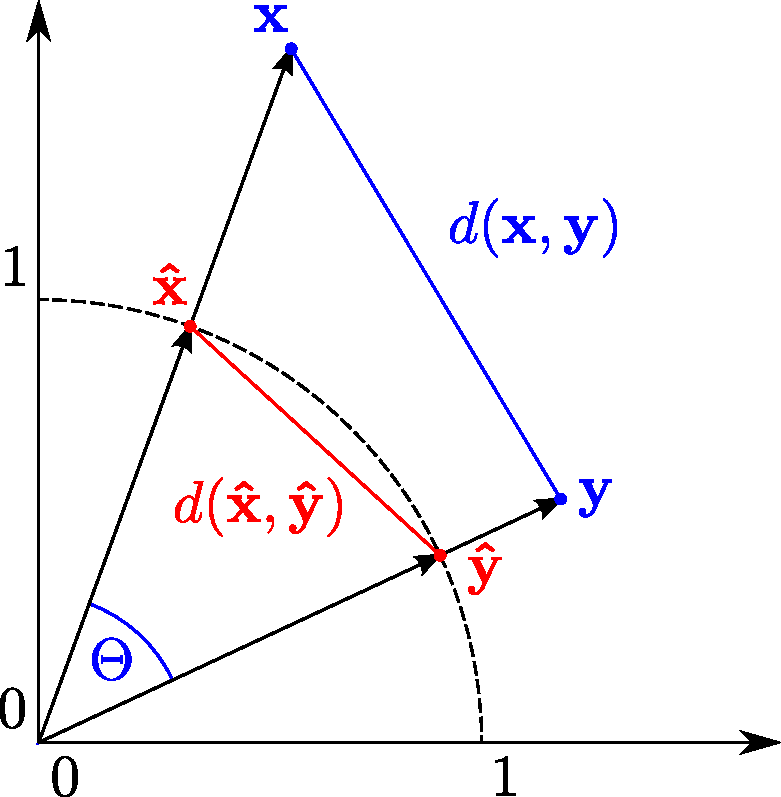
\includegraphics[width=\textwidth]{Graphics/L2.pdf}
    \end{subfigure}
    \caption[Chord Calculation Background]{\textbf{Chord Calculation Background.} The chord can be calculated with the radius similar for both vectors and the information of the angle of two vectors to the origin of the coordinate system. Since this information is not always available or sometimes expensive to calculate for a high number of vectors, the euclidean distance can be used with a L2-norm of both vectors equal to $r$ for similar results instead. To approximate cosine distance, the same calculation of euclidean distance is used with L2-norm equal to $r = 1$. To always obtain similar values of L2-norm equal to 1, L2-norm normalization is used on every vector.}
    \label{fig:L2_Normalisation_Background}
\end{figure}

\begin{equation}\label{eq:norm2}
    \begin{aligned}
        \mathbf{\hat{x}}_i = \frac{\mathbf{x}_i}{\Vert\mathbf{x}_i\Vert_2}
    \end{aligned}
\end{equation}

Calculation of chord distance $d_{\text{chord}}$ is possible when having two vectors, here as an example named as $\mathbf{x}'$ and $\mathbf{y}'$ with the same L2-norm equal to a radius $r$ of a sphere centered to the origin of the coordinate system and an angle of $\Theta'$ (\autoref{eq:chord} and \autoref{fig:L2_Normalisation_Background}). The euclidean distance $d_{\text{eucl}}$ is equal to the chord distance for the same vectors $\mathbf{x}'$ and $\mathbf{y}'$ with L2-norm of $r$.

\begin{equation}\label{eq:chord1}
    \Vert\mathbf{x}'\Vert_2 = \Vert\mathbf{y}'\Vert_2 = r \Rightarrow 
    \begin{aligned}
        d_{\text{chord}}(\mathbf{x}',\mathbf{y}') &= 2 \cdot r \sin \left(\frac{\Theta'}{2}\right)\\
        %&= 2 \cdot \frac{d_{\text{chord}}(\mathbf{x}',\mathbf{y}')}{2}\\
        %&= d_{\text{eucl}}(\mathbf{x}',\mathbf{y}')\\
        %&= \Vert\mathbf{x}' - \mathbf{y}'\Vert_2
    \end{aligned}
\end{equation}

Thus, in this project, chord distance can be calculated with the euclidean distance metric, posterior to the normalization with the L2-norm, which scales the vectors to the unit sphere.

\begin{equation}\label{eq:chord2}
    \Vert\mathbf{x}'\Vert_2 = \Vert\mathbf{y}'\Vert_2 = 1 \Rightarrow 
    \begin{aligned}
        d_{\text{chord}}(\mathbf{\hat{x}},\mathbf{\hat{y}}) &= d_{\text{eucl}}(\mathbf{\hat{x}},\mathbf{\hat{y}})\\
        &= \Vert\mathbf{\hat{x}} - \mathbf{\hat{y}}\Vert_2
    \end{aligned}
\end{equation}

The used chord distance is proportional with the initially intended to use cosine distance as shown in \autoref{eq:chord3}. Dividing the squared chord distance by 2 results in the cosine distance of the vectors.

\begin{equation}\label{eq:chord3}
    \Vert\mathbf{x}'\Vert_2 = \Vert\mathbf{y}'\Vert_2 = 1 \Rightarrow 
    \begin{aligned}  
        d_{\text{chord}}(\mathbf{\hat{x}},\mathbf{\hat{y}})^2 &= \Vert\mathbf{\hat{x}} - \mathbf{\hat{y}}\Vert_2^2\\
        &= (\mathbf{\hat{x}} - \mathbf{\hat{y}})^\top (\mathbf{\hat{x}} - \mathbf{\hat{y}})\\
        &= \mathbf{\hat{x}}^\top \mathbf{\hat{x}} - 2 \mathbf{\hat{x}}^\top \mathbf{\hat{y}} + \mathbf{\hat{y}}^\top \mathbf{\hat{y}}\\
        &= 2 - 2\mathbf{\hat{x}}^\top \mathbf{\hat{y}}\\
        &= 2 - 2 \cos(\Theta)\\
        &= 2 \cdot (1 - \cos(\Theta))\\
        &= 2 \cdot d_{\text{cos}}(\mathbf{x},\mathbf{y})
    \end{aligned}
\end{equation}

 Approximation of cosine distance by normalization with L2-norm followed by euclidean distance calculation is, thus, a possible and in this project used workaround, to overcome the impossibility to use cosine distance. 

%The default \colorbox{backcolour}{metric='euclidean'} setting was used for all following executions of \gls{HDBSCAN}, with an exception on the precalculated runs, to approximate the use of cosine distance metric as described in \autoref{sec:Normalization}. Therefore, matrix $\mathbf{X}_{\text{PCA}}$ and $\mathbf{Y}_{\text{UMAP}}$ have to be L2-norm normalized as described in \autoref{sec:Normalization} (\autoref{eq:l2_func_x} and \autoref{eq:l2_func_y}). For calculation of the linkage matrix $\mathbf{L}$, standard \gls{HDBSCAN} without $\varepsilon$ was used.

%\autoref{eq:HDB} to \autoref{eq:HDB_link_X} demonstrate the use of \gls{HDBSCAN} to calculate the linkage matrix $\mathbf{L}_{\text{PCA}}$ with matrix $\mathbf{X}_{\text{L2}}$ of \autoref{fig:Clustering_Pipeline} pathway \textsf{\textbf{1}} and was performed in the same way for $\mathbf{L}_{\text{UMAP}}$ with $\mathbf{Y}_{\text{L2}}$ of \autoref{fig:Clustering_Pipeline} pathway \textsf{\textbf{2}} \autocite{gower_minimum_1969, mcinnes_hdbscan_2017}.

% \begin{empheq}{alignat = -1}
%     &\mathbf{X}_{\text{L2}} &&= \text{NORMALIZE}_{\text{L2}}(\mathbf{X}_{\text{PCA}})\label{eq:l2_func_x}\\
%     &\mathbf{Y}_{\text{L2}} &&= \text{NORMALIZE}_{\text{L2}}(\mathbf{Y}_{\text{UMAP}})\label{eq:l2_func_y}
% \end{empheq}

% \begin{empheq}{alignat = -1}
%     &\mathbf{L}_{\text{PCA}} &&= \text{HDBSCAN}_{\text{Link}}(\mathbf{X}_{\text{L2}}, \text{min\_cluster\_size}, \text{min\_samples})\label{eq:HDB}\\
%     &&&= \text{HDBSCAN}_{\text{Link}}(\mathbf{X}_{\text{L2}}, 2, 1) \label{eq:HDB_link_X}
% \end{empheq}

Calculation of the chord distance by L2-norm normalized vectors euclidean distance is part of \glspl{HDBSCAN} mutual reachability distance calculation. The mutual reachability distance is the maximum of the chord distance and the core distances of two vectors (\autoref{eq:reach}). The core distance is the minimum radius necessary to include $k$ other vectors around a given vector. The standard setting of $k$ is five and not changed in this project \autocite{mcinnes_hdbscan_2017}. 

% \begin{empheq}{alignat = -1}
%     &d_{\text{mreach}-k}(\mathbf{x},\mathbf{y}) &&= \max \{ \text{core}_k(\mathbf{x}), \text{core}_k(\mathbf{y}), d_{\text{eucl}}(\mathbf{x},\mathbf{y}) \} \label{eq:reach}
% \end{empheq}

\begin{figure}[!hbt]
    \centering
    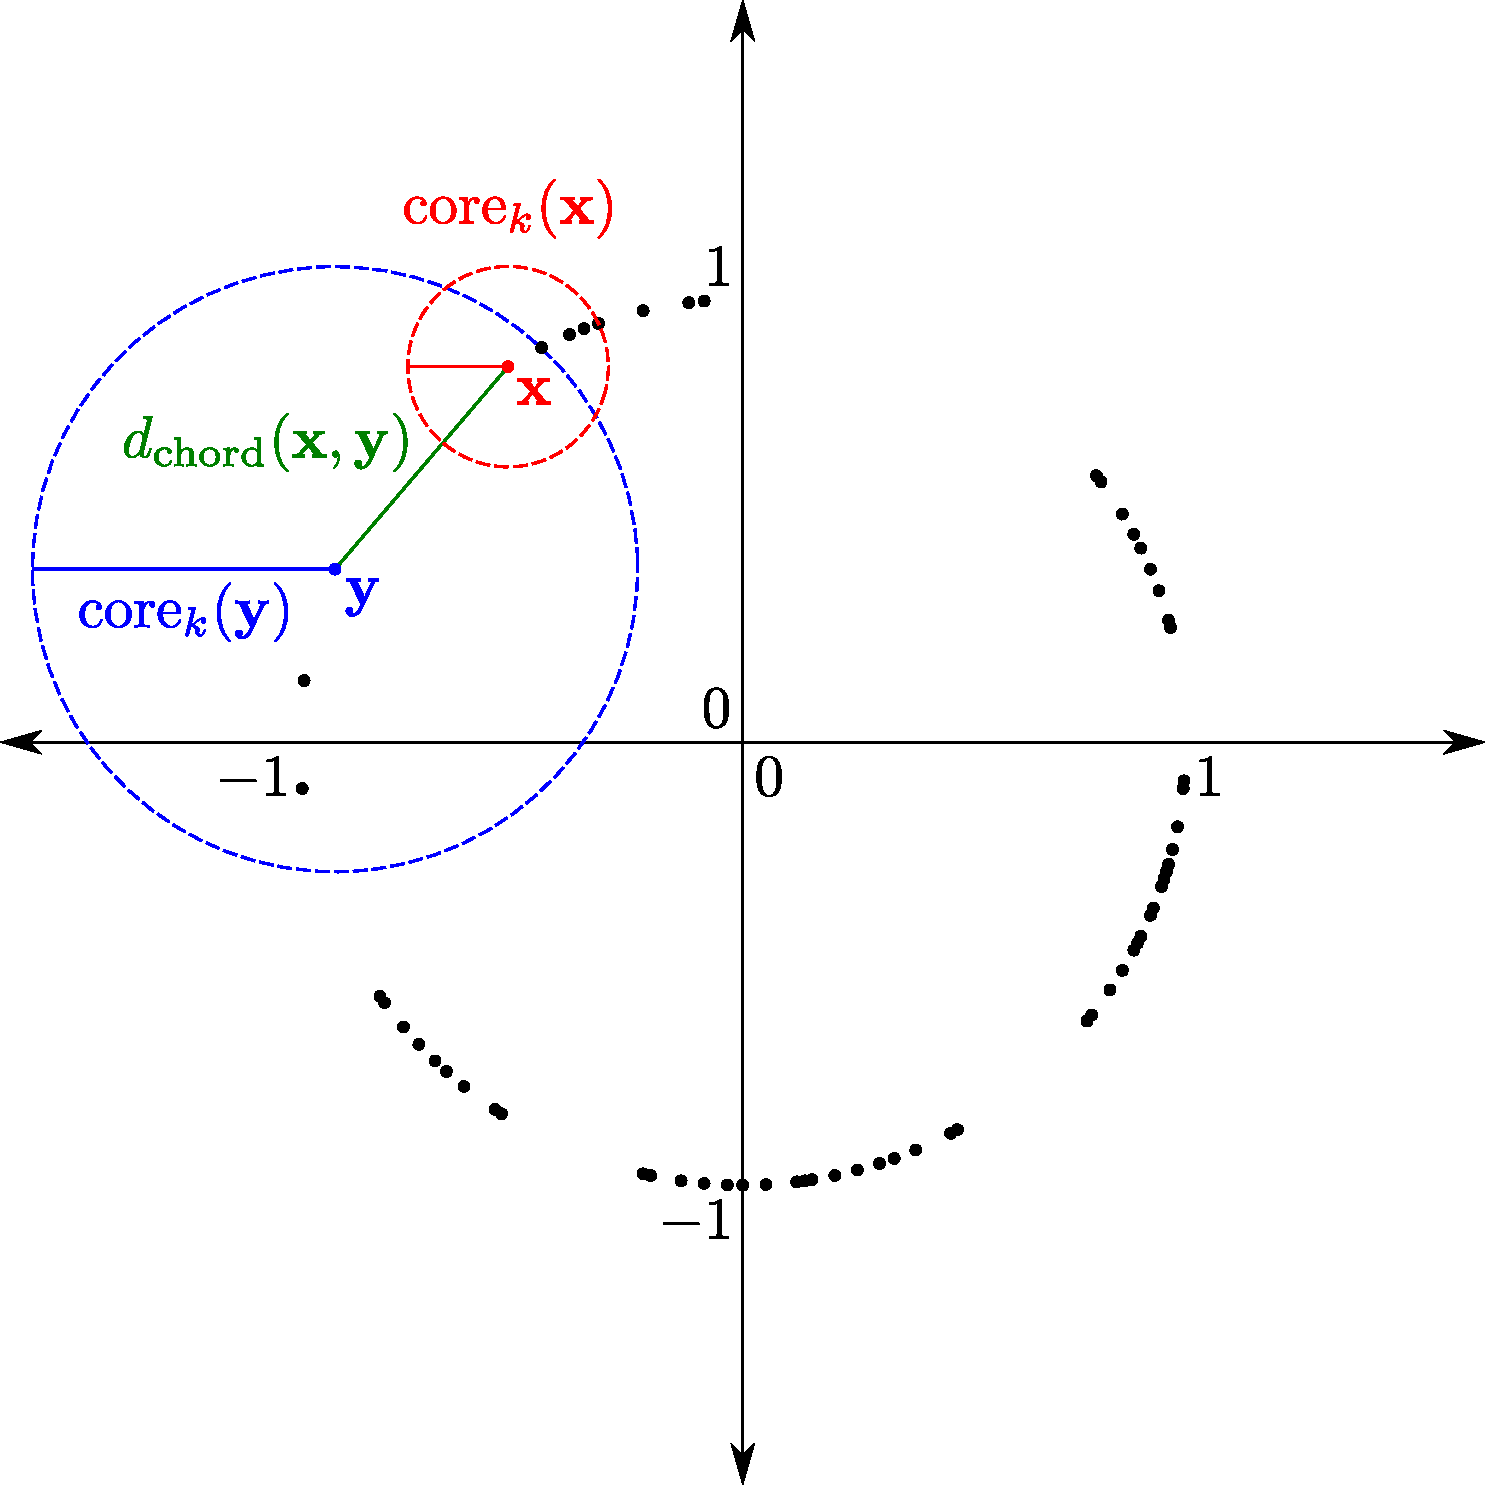
\includegraphics[width=\textwidth]{Graphics/HDB.pdf}
    \caption[Mutual Reachability Calculation]{\textbf{Mutual Reachability Calculation.} A low dimension representation of the calculation \gls{HDBSCAN} performed in this project. To calculate the mutual reachability distance, a radius is measured necessary to include the next five points, as example for vector $\mathbf{x}$ in blue and $\mathbf{y}$ in red. The euclidean distance between these vectors is then calculated and compared to the radii. The maximum of both radii and the euclidean distance is the mutual reachability distance (\autoref{eq:reach}).}
    \label{fig:HDB}
\end{figure}


\begin{figure}[!hbt]
    \centering
    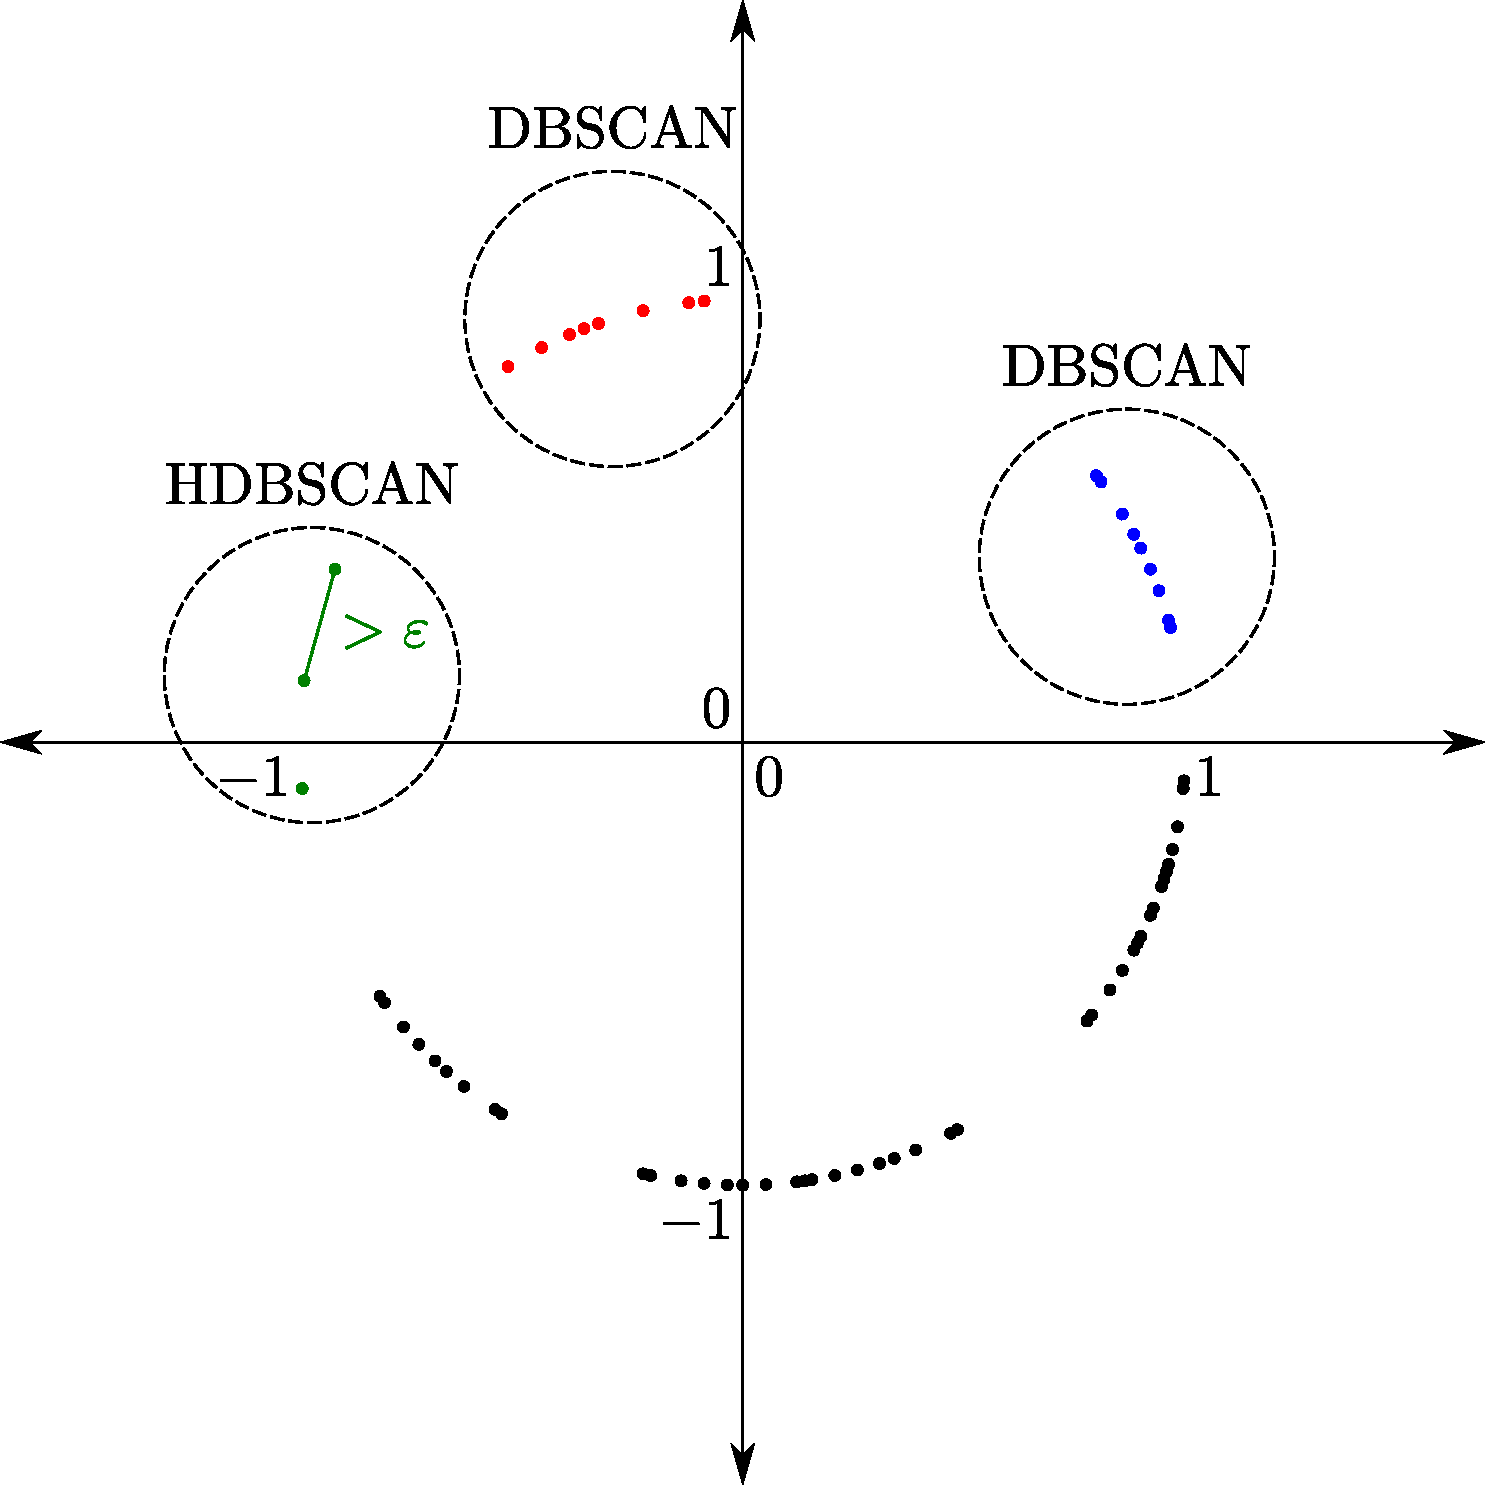
\includegraphics[width=\textwidth]{Graphics/Hybrid.pdf}
    \caption[Hybrid Clustering Threshold]{\textbf{Hybrid Clustering Threshold.} The hybrid clustering differentiate between clusters where points are connected by distances smaller and higher than $\varepsilon$. When the distance is smaller, the \gls{DBSCAN} algorithm is used and clusters are calculated based on this threshold value $\varepsilon$ by combining points with less distance. For single points, having no point in reachable distance and, therefore, impossible to be clustered by \gls{DBSCAN}, other than single sequence cluster, \gls{HDBSCAN} is used to builds cluster with higher threshold if appropriate. The graphic is based on \glqq Combining HDBSCAN* with DBSCAN\grqq{} in the \href{https://hdbscan.readthedocs.io/en/latest/api.html}{API} adapted to the calculations in this project, as two dimensional example.}
    \label{fig:Hybrid}
\end{figure}

To find an appropriate value for $\varepsilon$, two different methods were used and compared (\autoref{fig:Clustering_Pipeline} pathway \textsf{\textbf{3}} and \textsf{\textbf{4}}. Using the first method, the \gls{DBCV} exploration in \autoref{fig:Clustering_Pipeline} \textsf{\textbf{G}}, execution of \gls{HDBSCAN} was repeated with different settings for $\varepsilon$ and compared by the \gls{DBCV} to find the value of $\varepsilon$ that maximizes the \gls{DBCV} \autocite{moulavi_density-based_2014}. For these repeated executions of \gls{HDBSCAN}, \colorbox{backcolour}{gen\_min\_span\_tree=True} setting was also necessary, to be able to calculate the \gls{DBCV} with the minimum spanning tree (\autoref{eq:DBCV_X}) \autocite{moulavi_density-based_2014, gower_minimum_1969}. The exploration was executed for $\mathbf{X}_{\text{L2}}$ and $\mathbf{Y}_{\text{L2}}$ to find the optimal $\varepsilon_{\text{PCA}}$ and $\varepsilon_{\text{UMAP}}$.

% \begin{empheq}{alignat = -1}
%     &\max_{\substack{0 \leq \varepsilon}} \left(\text{HDBSCAN}_{\text{DBCV}}(\mathbf{X}_{\text{L2}}, 2, 1, \varepsilon)\right) = \text{HDBSCAN}_{\text{DBCV}}(\mathbf{X}_{\text{L2}}, 2, 1, \varepsilon') \Rightarrow \varepsilon' = \varepsilon_{\text{PCA}} \label{eq:DBCV_X}
% \end{empheq}

Using the second method, the optimal value for $\varepsilon_{\text{UMAP'}}$ and $\varepsilon_{\text{PCA'}}$ were calculated using the Kneedle Algorithm \autoref{sec:Kneedle} \autocite{halko_finding_2010}.

With the optimal values for $\varepsilon$ found by \gls{DBCV} exploration and the Kneedle Algorithm, as well as with the matrix for the \gls{UMAP} settings and the one for the \gls{PCA} settings, \gls{HDBSCAN} with the hybrid clustering setting was executed four times. Each execution resulted in the mathematical sequence of cluster names $N$ related to the sequence of genomic sequences $S$ (\autoref{eq:HDB_cluster_PK} to \autoref{eq:HDB_cluster_UD}) (\autoref{fig:Clustering_Pipeline} \textsf{\textbf{H}}) \autocite{mcinnes_hdbscan_2017, malzer_hybrid_2020}. To sum it up, with the \acrshort{UMAP}/\acrshort{DBCV} method, the cluster name of the first genomic sequence of $S$ is the first element of mathematical sequence $N_{\text{UMAP}}$. 

% \begin{empheq}{alignat = -1}
%     &N_{\text{PCA}} &&= \text{HDBSCAN}_{\text{Hybrid}}(\mathbf{X}_{\text{L2}}, 2, 1, \varepsilon_{\text{PCA}}) \label{eq:HDB_cluster_PK}\\
%     &N_{\text{UMAP}} &&= \text{HDBSCAN}_{\text{Hybrid}}(\mathbf{Y}_{\text{L2}}, 2, 1, \varepsilon_{\text{UMAP}}) \label{eq:HDB_cluster_UK}\\
%     &N_{\text{PCA'}} &&= \text{HDBSCAN}_{\text{Hybrid}}(\mathbf{X}_{\text{L2}}, 2, 1, \varepsilon_{\text{PCA'}}) \label{eq:HDB_cluster_PD}\\
%     &N_{\text{UMAP'}} &&= \text{HDBSCAN}_{\text{Hybrid}}(\mathbf{Y}_{\text{L2}}, 2, 1, \varepsilon_{\text{UMAP'}}) \label{eq:HDB_cluster_UD}
% \end{empheq}

% Important parameters used in this project, including settings varying from the default, are listed below. All available settings with explanation are listed in the \href{https://hdbscan.readthedocs.io/en/latest/api.html}{API}.

% \begin{leftbar}
%     \textbf{hdbscan.HDBSCAN}
%     \begin{nstabbing}
%         \qquad\qquad\qquad\qquad\qquad\quad\=\kill

%         min\_cluster\_size \> [min. size of a cluster (default: 5)]\\
        
%         min\_samples \> [conservativeness of the clustering (default: None)]\\
        
%         cluster\_selection\_epsilon \> [merge clusters below the threshold (default: 0.0)]\\
        
%         gen\_min\_span\_tree \> [generate the minimum spanning tree (default: False)]\\
        
%         metric \> [metric to use for clustering (default: euclidean)]
%         %alpha \> (default: 1.0)
%     \end{nstabbing}
% \end{leftbar}

%Clustering
%DBCV mehr als 50dims abkacken bla
%Metrik
%Hybrid selection
%Needle
%Linkage matrix

\section{Kneedle Algorithm} \label{sec:Kneedle}

Calculation of $\varepsilon$ was executed by using the implementation of the Kneedle Algorithm proposed in the associated \href{https://github.com/arvkevi/kneed.git}{GitHub repository} \autocite{satopaa_finding_2011}.

Points where e.~g.~ the cost of tuning is no longer worth the loss in performance are called \glqq knees\grqq{} \autocite{satopaa_finding_2011}. These points are so to speak the balance of a given trade-off \autocite{satopaa_finding_2011}. Kneedle is an algorithm to find these point in a given system \autocite{satopaa_finding_2011}. A system could be the trade-off between cluster number and distance threshold in hierarchical clustering \autocite{gower_minimum_1969}. 

With increasing cluster number, the distance threshold of hierarchical clustering decreases \autocite{gower_minimum_1969}. This describes a decreasing curve of convex type with distance threshold on the y- and cluster number on the x-axis. The knee is the number of clusters at the point in the polynomial representation of the curve with maximal acceleration. Polynomial representation was used to find the maximum acceleration of the smoothed curve, instead of a local maximum due to a single inaccuracy. Therefore the implementation Kneed was used with \colorbox{backcolour}{curve='concave'}, \colorbox{backcolour}{direction='increasing'} and \colorbox{backcolour}{interp\_method='interp1d'} settings \autoref{fig:Clustering_Pipeline} \textsf{\textbf{I}}).

\begin{empheq}{alignat = -1}
    &n &&= \text{KNEED}(\mathbf{L})
\end{empheq}

Number of clusters $n$ was then converted in it's respective distance threshold $\varepsilon$ using the linkage matrix $\mathbf{L}$ again.

The parameters used in this project with settings varying from the default are listed below. All available settings can be fount in the \href{https://kneed.readthedocs.io/en/stable/api.html}{API}.

\begin{leftbar}
    \textbf{kneed.KneeLocator}
    \begin{nstabbing}
        \qquad\qquad\qquad\qquad\qquad\quad\=\kill

        x \> \\
        
        y \> \\
        
        curve \> (default: 'concave')\\
        
        direction \> (default: 'increasing')\\
        
        interp\_method \> (default: 'interp1d')\\
        
        online \> (default: False)\\
        
        %S \> (default: 1.0)\\
        %polynomial\_degree \> (default: 7)
    \end{nstabbing}
\end{leftbar}



\section{Biopython \& Scipy} \label{sec:MAFFT}

The colored trees were created by \textbf{ETE3} with a newick file created with $N_{\text{PCA}}$ or $N_{\text{PCA'}}$ and $\mathbf{L}_{\text{PCA}}$ and otherwise $N_{\text{UMAP}}$ or $N_{\text{UMAP'}}$ and $\mathbf{L}_{\text{UMAP}}$ (\autoref{fig:PCA_Clusteree_Knee_4}, \autoref{fig:UMAP_Clusteree_Knee_4}) \autocite{huerta-cepas_ete_2016}. The newick file was created with a feature request proposed for the \textbf{scipy} package version 1.6.0 involving the \textbf{cluster.hierarchy.to\_tree} function as described in the \href{https://github.com/scipy/scipy/issues/8274}{issue}\footnote{last accessed 02/06/21} (\autoref{fig:Tree_Pipeline} \textsf{\textbf{J}}) \autocite{scipy_10_contributors_scipy_2020}.

\begin{leftbar}
    %\textbf{mafft}
    \textbf{scipy.cluster.hierarchy.to\_tree}
    \begin{nstabbing}
        \qquad\qquad\qquad\qquad\qquad\quad\=\kill
    
        Z \> [input linkage matrix]
    \end{nstabbing}
\end{leftbar}

For choosing all the clusters centroid sequences $C$ which are a subset of all the genomic sequences $S$, the \textbf{spatial.distance.cdist} function also from the \textbf{scipy} package was used (\autoref{fig:Tree_Pipeline} \textsf{\textbf{K}}) \autocite{scipy_10_contributors_scipy_2020}. Let $S_{\text{Clst}}$ be the subset of $S$ matching the sequences belonging to cluster $o$ in $N$ and $\mathbf{X}_{\text{Clst}}$ the L2-norm normalized matrix of $S_{\text{Clst}}$ and therefore a portion of $\mathbf{X}_{\text{L2}}$. The centroid sequence $C_o$ of the cluster $o$ is the sequence $S_i$ of $S_{\text{Clst}}$ where sum of the cosine distance of vector representation $\mathbf{x}_i$ to all the other $k$ vectors of $\mathbf{X}_{\text{Clst}}$ is equal the minimum of the \textbf{spatial.distance.cdist} function with the normalized matrix $\mathbf{X}_{\text{Clst}}$ of $S_{\text{Clst}}$ and \colorbox{backcolour}{metric='euclidean'} \autoref{eq:centroid}.

\begin{empheq}{alignat = -1}
    &\min \left( \text{CDIST}_{\text{eucl}}(\mathbf{X}_{\text{Clst}}, \mathbf{X}_{\text{Clst}}) \right) &&= \sum^k_{j=1} d_{\text{eucl}}(\mathbf{x}_i, \mathbf{x}_j ) \Rightarrow C_o = S_i\label{eq:centroid}
\end{empheq}

For the pairwise alignments in \autoref{sec:Serotype_Classification} from the \textbf{biopython (Bio)} package version 1.78 the \textbf{Align.PairwiseAligner} function was used with standard settings \autocite{cock_biopython_2009}. 

Important parameters used in this project including settings varying from the default are listed below. All available settings can be fount in the \href{https://biopython.org/docs/1.75/api/Bio.Align.html}{API}.

\begin{leftbar}
    %\textbf{mafft}
    \textbf{Bio.Align.PairwiseAligner}
    \begin{nstabbing}
        \qquad\qquad\qquad\qquad\qquad\quad\=\kill
    
         seqA \> [Input sequence A]\\ 
         
         seqB \> [Input sequence B]
        
        %-{}-{}6merpair \> (default: on)\\
        %\> input\\
        %> \> output
    \end{nstabbing}
\end{leftbar}

The materials named in the following are only used for the analyses in the \autoref{sec:Clustering_Anomalies} to \autoref{sec:Dimension_Reduction} and therefore not part of the proposed raw clustering tool (\autoref{fig:Alignment_Pipeline} and \autoref{fig:Precalc_Pipeline}).

\begin{figure}[!hbt]
    \centering
    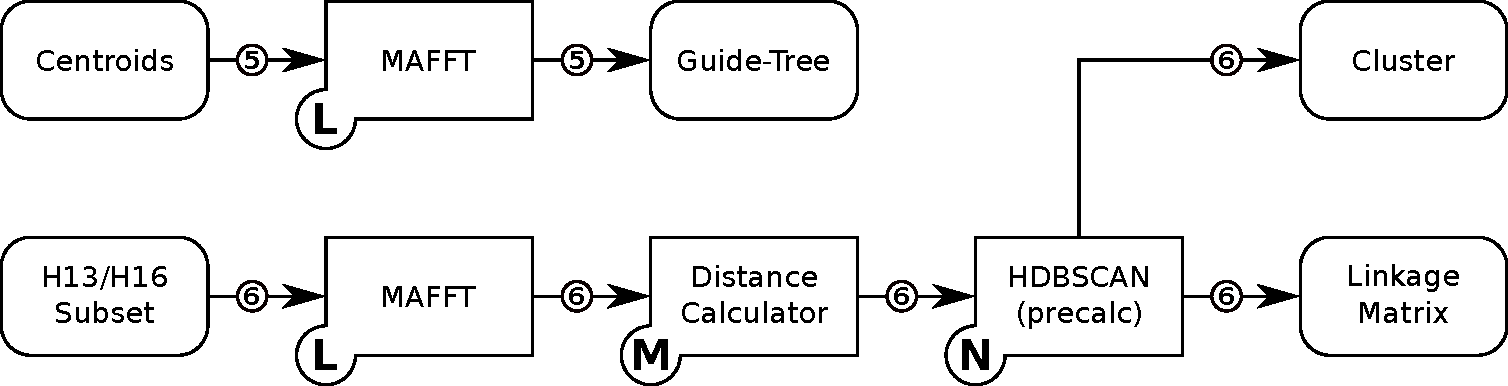
\includegraphics[width=\textwidth]{Graphics/Alignment.pdf}
    \caption[Alignment Pipeline]{\textbf{Alignment Pipeline.} The analysis steps involving \glspl{MSA} are performed as pictured. The sequences related to the centroids were aligned using MAFFT resulting in the output as guide-tree visualized by \textbf{ETE3}. The small subset for comparison was also aligned by MAFFT prior to evolutionary distance calculation and clustering by \gls{HDBSCAN}.}
    \label{fig:Alignment_Pipeline}
\end{figure}

\begin{figure}[!hbt]
    \centering
    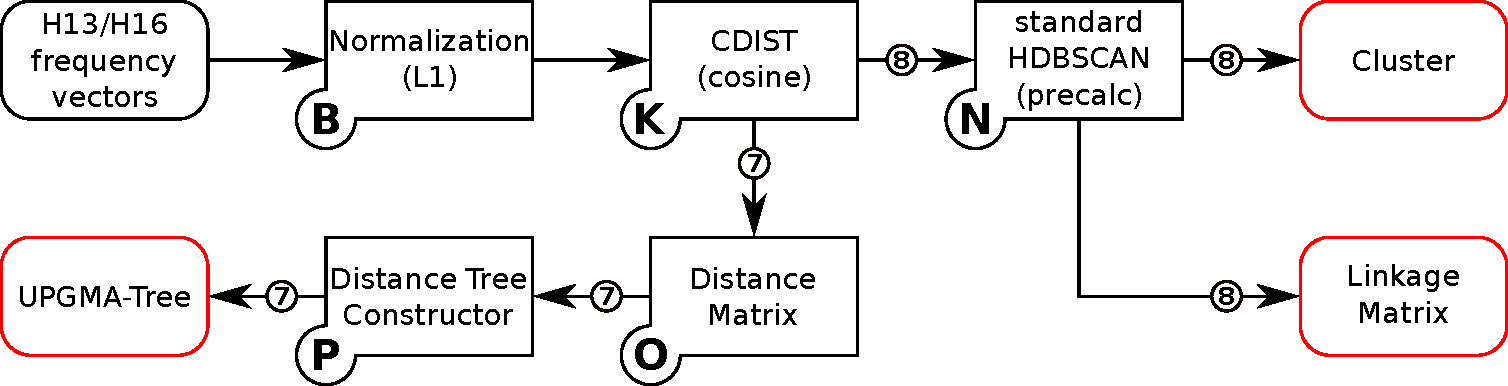
\includegraphics[width=\textwidth]{Graphics/Precalculated.pdf}
    \caption[Precalculation Pipeline]{\textbf{Precalculation Pipeline.} For the precalculated trees the L1-normalized k-mer vectors were compared by cosine distance prior to clustering by \gls{HDBSCAN} and on the other hand processing with \textbf{biopython (Bio)} package \gls{UPGMA} calculation and visualization by \textbf{ETE3}.}
    \label{fig:Precalc_Pipeline}
\end{figure}

The Biopython implementation of MAFFT version 7.475 from the \textbf{biopython (Bio)} package version 1.78 was used to build the guide trees in \autoref{sec:Clustering_Anomalies} according to \autoref{fig:Alignment_Pipeline} pathway \textsf{\textbf{5}} with the genomic sequences of the centroids $C$ \autocite{katoh_mafft_2013, cock_biopython_2009} (\autoref{fig:Alignment_Pipeline}. The settings were mostly the default settings proposed in the \href{https://mafft.cbrc.jp/alignment/software/}{manual}. For faster execution \colorbox{backcolour}{thread=6} and for export of the guide tree \colorbox{backcolour}{treeout=True} setting was used \autocite{katoh_mafft_2013, cock_biopython_2009}. The guide-tree was colored with \textbf{ETE3} (\autoref{fig:Alignment_Pipeline} \textsf{\textbf{K}}) \autocite{huerta-cepas_ete_2016}.

Important parameters used in this project including settings varying from the default are listed below. All available settings can be fount in the \href{https://mafft.cbrc.jp/alignment/software/}{manual}.

\begin{leftbar}
    %\textbf{mafft}
    \textbf{Bio.Align.Applications.MafftCommandline}
    \begin{nstabbing}
        \qquad\qquad\qquad\qquad\qquad\quad\=\kill
    
        treeout \> [export guide tree used for alignment (default: off)]\\
        
        thread \> [number of used threads (default: 1)]\\
        
        input \> [input FASTA file]
        
        %-{}-{}6merpair \> (default: on)\\
        %\> input\\
        %> \> output
    \end{nstabbing}
\end{leftbar}

In \autoref{sec:Comparison_Clustering} five different cluster trees are compared to each other. The trees are based on clustering with \gls{HDBSCAN}, without hybrid clustering ($\varepsilon=0$) \autocite{malzer_hybrid_2020, mcinnes_hdbscan_2017}. For each clustering a different matrix was used as input. The trees of \gls{UMAP} and \gls{PCA} (\autoref{fig:Simple_Clustertree_PCA} and \autoref{fig:Simple_Clustertree_UMAP}) were created according to \autoref{fig:Vectorization_Pipeline} and \autoref{fig:Clustering_Pipeline} and as described in \autoref{sec:Frequency} to \autoref{sec:HDBSCAN} with a smaller FASTA subset $S$ containing only segment 4 sequences with subtypes H13 and H16 and a resulting smaller L2-norm normalized \gls{PCA} matrix $\mathbf{X}_{\text{L2}}$ and smaller \gls{UMAP} matrix $\mathbf{Y}_{\text{L2}}$. Clustering for the trees of \gls{UMAP} and \gls{PCA} was performed similar to \autoref{sec:HDBSCAN} but without $\varepsilon$ with the small matrix variants of $\mathbf{X}_{\text{L2}}$ and $\mathbf{Y}_{\text{L2}}$ (\autoref{eq:hdb_prime_x} and \autoref{eq:hdb_prime_y}). 

\begin{empheq}{alignat = -1}
    &N_{\text{UMAP}} &&= \text{HDBSCAN} (\mathbf{X}_{\text{L2}}, 2, 1, 0)\label{eq:hdb_prime_x}\\
    &N_{\text{PCA}} &&= \text{HDBSCAN} (\mathbf{Y}_{\text{L2}}, 2, 1, 0)\label{eq:hdb_prime_y}
\end{empheq}

The two trees based the clustering with precalculation (\autoref{fig:Simple_Clustertree_Cosine} and \autoref{fig:Simple_Clustertree_Euclid}) were created by distance calculation on the L1-norm normalized matrix $\mathbf{X}_{\text{L1}}$ of the smaller $S$. For the calculation of the distance the \textbf{scipy} package version 1.6.0 was used with the \textbf{spatial.distance.cdist} function (\autoref{fig:Precalc_Pipeline} \textsf{\textbf{N}}) \autocite{scipy_10_contributors_scipy_2020}. For calculation of the cosine distance \colorbox{backcolour}{metric='cosine'} and for euclidean distance \colorbox{backcolour}{metric='euclidean'} setting was used (\autoref{eq:c_calc_matrix} to \autoref{eq:e_calc_matrix}). The resulting distance matrices $\mathbf{C}$ and $\mathbf{E}$ were clustered with \gls{HDBSCAN} and \colorbox{backcolour}{metric='precalculated'} setting (\autoref{fig:Precalc_Pipeline} \textsf{\textbf{F}} and \autoref{eq:hdb_prime_e} to \autoref{eq:hdb_prime_c}) \autocite{mcinnes_hdbscan_2017}.

% \begin{empheq}{alignat = -1}
%     &c_{i,j} &&= d_{\text{cos}}(\mathbf{x}_i, \mathbf{x}_j), \ i = 1, \ldots o, \ j = 1, \ldots o\label{eq:c_calc_1}\\
%     &&&= 1 - \frac{\mathbf{x}_i^\top\mathbf{x}_j}{\Vert\mathbf{x}_i\Vert \cdot \Vert\mathbf{x}_j\Vert}\label{eq:c_calc_2}
% \end{empheq}

\begin{empheq}{alignat = -1}
    &\mathbf{C} &&= \text{CDIST}_{\text{cosine}}(\mathbf{X}_{\text{L1}}, \mathbf{X}_{\text{L1}}) \label{eq:c_calc_matrix}\\
    &\mathbf{E} &&= \text{CDIST}_{\text{euclidean}}(\mathbf{X}_{\text{L1}}, \mathbf{X}_{\text{L1}}) \label{eq:e_calc_matrix}
\end{empheq}

\begin{empheq}{alignat = -1}
    &N_{\text{eucl}} &&= \text{HDBSCAN} (\mathbf{E}, 2, 1, 0)\label{eq:hdb_prime_e}\\
    &N_{\text{cos}} &&= \text{HDBSCAN} (\mathbf{C}, 2, 1, 0)\label{eq:hdb_prime_c}
\end{empheq}

Important parameters used in this project including settings varying from the default are listed below. All available settings can be fount in the \href{https://docs.scipy.org/doc/scipy/reference/generated/scipy.spatial.distance.cdist.html}{API}.

\begin{leftbar}
    \textbf{scipy.spatial.distance.cdist}
    \begin{nstabbing}
        \qquad\qquad\qquad\qquad\qquad\quad\=\kill
    
        metric \> [Distance metric for calculation (default: 'euclidean')]

    \end{nstabbing}
\end{leftbar}

The \textbf{spatial.distance.cdist} function is also used for a fast pairwise alignment using the mentioned \textbf{Align.PairwiseAligner} above. Therefore a small python definition containing the \textbf{Align.PairwiseAligner} function was inserted as metric setting into \textbf{spatial.distance.cdist}. 

The last of the five trees is based on MAFFT with the \textbf{biopython} package. The alignment was done on the subset $S$. On the alignment the distance matrix was calculated by the \textbf{Phylo.TreeConstruction.DistanceCalculator} function from the \textbf{biopython (Bio)} package. The standard settings for nucleotide sequences was used for the calculation \colorbox{backcolour}{model='identity'} \autocite{cock_biopython_2009}.

\begin{empheq}{alignat = -1}
    &\mathbf{G} &&= \text{DistanceCalculator}_{\text{identity}}(\text{MAFFT}(S_{\text{Sub}}))
\end{empheq}

\begin{empheq}{alignat = -1}
    &N_{\text{msa}} &&= \text{HDBSCAN} (\mathbf{G}, 2, 1, 0)\label{eq:hdb_prime_g}\\
\end{empheq}

Important parameters used in this project including settings varying from the default are listed below. All available settings can be fount in the \href{https://biopython.org/docs/latest/api/Bio.Phylo.TreeConstruction.html}{API}.

\begin{leftbar}
    \textbf{Bio.Phylo.TreeConstruction.DistanceCalculator}
    \begin{nstabbing}
        \qquad\qquad\qquad\qquad\qquad\quad\=\kill
    
        model \> [model for distance calculation (default: 'identity')]

    \end{nstabbing}
\end{leftbar}

The \textbf{Phylo.TreeConstruction.DistanceMatrix} and \textbf{DistanceTreeConstructor} function also from the \textbf{biopython} package was used for calculation of precalculated UPGMA trees in \autoref{sec:K_mer_Representation}. Instead of the default neighbor joining setting, the bottom-up hierarchical clustering method \colorbox{backcolour}{method='upgma'} was used (\autoref{fig:Alignment_Pipeline} \textsf{\textbf{O}} and \textsf{\textbf{P}}) \autocite{gower_minimum_1969, cock_biopython_2009}. The matrices calculated in \autoref{eq:c_calc_matrix} and \autoref{eq:e_calc_matrix} were used as input for the calculation of the UPGMA-trees \autocite{sokal_statistical_1958}.

Important parameters of both tools used in this project including settings varying from the default are listed below. All available settings can be fount in the same \href{https://biopython.org/docs/latest/api/Bio.Phylo.TreeConstruction.html}{API} of \textbf{Bio.Phylo.TreeConstruction}.

\begin{leftbar}
    \textbf{Bio.Phylo.TreeConstruction.DistanceMatrix}
    \begin{nstabbing}
        \qquad\qquad\qquad\qquad\qquad\quad\=\kill
    
        names \> [name of columns and rows]\\
        
        matrix \> [input matrix]
    \end{nstabbing}
\end{leftbar}

\begin{leftbar}
    \textbf{Bio.Phylo.TreeConstruction.DistanceTreeConstructor}
    \begin{nstabbing}
        \qquad\qquad\qquad\qquad\qquad\quad\=\kill
    
        method \> [construction method for the distance tree (default: 'nj')]
        
    \end{nstabbing}
\end{leftbar}